\chapter{Teorema de Fatou y Teorema de Carathéodory}

\begin{comment}
    \begin{theorem}[Lema de Schwart]
        Sea $f: \disk \to \closedisk$ una función $\in \holomorphic{\disk}$ tal que $f(0) = 0$. Entonces:
        \begin{itemize}
            \item $\abs{f(z)} \leq \abs{z}$ para todo $z \in \disk$.
            \item Si para algún $z_0 \not = 0$ tenemos que $\abs{f(z_0)} = \abs{z_0}$, entonces existe $\alpha \in \complex, \abs{\alpha} = 1$ tal que $f(z)=\alpha z$.
        \end{itemize}
    \end{theorem}

    \begin{proof}
        Sea $f(z) = a_1z + \cdots$ la serie de potencias de $f$. El término constante es $0$ puesto que suponemos que $f(0) = 0$. Entonces $f(z)/z$ es una función holomorfa y
        \begin{equation*}
            \abs{\dfrac{f(z)}{z}} < 1/r \text{ para } \abs{z} = r < 1
        \end{equation*}
    \end{proof}
\end{comment}

Para empezar vamos a realizar una pequeña introducción a la integral de Poisson. A continuación probaremos el Teorema de Fatou para límites radiales. Por último hablaremos sobre aplicaciones conformes y demostraremos el Teorema de Carathéodory. \\

\section{La Integral de Poisson}

\begin{definition}
    Se llama núcleo de Poisson a la función $P$ definida por
    \begin{equation}
        \label{poisson1}
        P:(r,t) \in [0,1)\times \real \mapsto P_r(t) = \sum_{n=-\infty}^{\infty} r^{\abs{n}}e^{int}.
    \end{equation}

    Podemos considerar el núcleo de Poisson como una función de dos variables $r$ y $t$ o como una familia de funciones de $t$ que dependen de $r$. \\

    Dado $z = re^{i \theta}$, con $r \in [0,1)$ y $\theta \in \real$ se tiene que
    \begin{equation} \label{poisson2}
        P_r(\theta - t) =  \dfrac{1 - r^2}{1 - 2r \cos (\theta - t) + r^2} = \Re \left[ \dfrac{e^{it} + z}{e^{it} - z} \right]
    \end{equation}
    para todo $t \in \real$. En efecto:
    \begin{equation*}
        \begin{split}
            P_r(t) & = \sum_{n=-\infty}^{\infty} r^{\abs{n}}e^{int} = 1 + \sum_{n=1}^{\infty} r^n e^{int} + \sum_{n=1}^{\infty} r^n e^{-int} = 1 + \sum_{n=1}^{\infty} r^n (e^{int} + e^{-int}) = \\
                   & =  1 + \sum_{n=1}^{\infty} r^n 2 \Re(e^{int}) = \Re \left[ 1 + 2 \sum_{n=1}^{\infty} (r e^{it})^n  \right] = \Re \left[ 1 + 2 \dfrac{re^{it}}{1-re^{it}} \right] = \Re \left[\dfrac{1 + re^{it}}{1-re^{it}} \right].
        \end{split}
    \end{equation*}

    Por otra parte,
    \begin{equation} \label{poisson3}
        \Re \left[ \dfrac{1 + re^{it}}{1-re^{it}} \right] = \Re \left[ \dfrac{(1 + re^{it})(1 - re^{it})}{\abs{1-re^{it}}^2} \right] = \dfrac{1 - r^2}{1 - 2r \cos t + r^2}.
    \end{equation}
    así que
    \begin{equation} \label{poisson4}
        P_r(t) =  \dfrac{1 - r^2}{1 - 2r \cos t + r^2} = \Re \left[ \dfrac{1 + re^{it}}{1 - re^{it}} \right]. % Para pasar de esta ecuación a la primera se multiplica y divide por e^{it}
    \end{equation}
\end{definition}
\medskip

\begin{prop}{El núcleo de Poisson satisface las siguientes propiedades:}
    \label{properties}
    {
    \leqnomode
    \setlength{\jot}{15pt}
    \setlength{\mathindent}{30pt}
    \begin{align}
        & \dfrac{1}{2 \pi} \int_{- \pi}^{\pi} P_r (t) dt = 1;
        \alignno \label{property1} \\
        & P_r(t) > 0 \text{ para todo } t \in \real;
        \alignno \label{property2} \\
        & P_r(t) = P_r(-t) \text{ para todo } t \in \real, \text{ y } P_r(t) \text{ es periódica en } t \text{ de periodo } 2 \pi;
        \alignno \label{property3} \\
        & P_r(t) < P_r(\delta) \text{ si } 0 < \delta < \abs{t} \leq \pi;
        \alignno \label{property4}\\
        & \lim_{r \to 1^-} P_r(\delta) = 0 \text{ para todo } \delta \in (0, \pi].
        \alignno \label{property5}
    \end{align}
    }
\end{prop}

\begin{proof}
    \eqref{property1} Dado $r, \, 0 \leq r < 1$, la serie \ref{poisson1} converge uniformemente en $t$. Así que
    \begin{equation*}
        \dfrac{1}{2 \pi} \int_{- \pi}^{\pi} P_r (t) dt  = \dfrac{1}{2 \pi} \int_{- \pi}^{\pi} \sum_{n=-\infty}^{\infty} r^{\abs{n}}e^{int} dt = \dfrac{1}{2 \pi} \sum_{n=-\infty}^{\infty} r^{\abs{n}} \int_{- \pi}^{\pi} e^{int} dt = 1.
    \end{equation*}

    \eqref{property2} De las ecuaciones \eqref{poisson3} y \eqref{poisson4}, tenemos que $P_r(t) = (1- r^2) \abs{1 - re^{it}}^{-2} > 0$ ya que $r < 1$. \\

    \eqref{property3} Es consecuencia trivial de la expresión \eqref{poisson4}. \\

    \eqref{property4} Fijados $r$, $\delta$ y $t$ en las condiciones indicadas se verifica que $\cos t < \cos \delta$, de donde se sigue que $P_r(t) < P_r(\delta)$. \\

    \eqref{property5} De la ecuación \eqref{poisson4}, tenemos que $\lim_{r \to 1^-} (1 - r^2) = 0$ y $\lim_{r \to 1^-} (1 - 2r \cos \delta + r^2) \not = 0$ así que $\lim_{r \to 1^-} P_r() = 0$. \\
\end{proof}

\begin{definition}
    Se llama integral de Poisson de una función $f \in L^1(\partial \disk)$ a la función $F$ dada por
    \begin{equation*}
        F: z=re^{i \theta} \in \disk \mapsto F(re^{i \theta}) = \dfrac{1}{2 \pi} \int_{- \pi}^{\pi} P_r (\theta - t) f(e^{it}) dt.
    \end{equation*}

    Algunas veces nos convendrá referirnos a ella como $F = P[f]$.
\end{definition}

Además si $f$ lleva $\partial \disk$ en los reales, \ref{poisson2} nos muestra que % extender esto
\begin{equation*}
    P[f] = \Re \left[ \dfrac{1}{2} \int_{-\pi}^{\pi} \dfrac{e^{it} + z}{e^{it} - z} f(e^{it}) dt \right].
\end{equation*}

También haciendo el cambio de variable $\theta - t = x$ se tiene la igualdad
\begin{equation*}
    F(re^{i \theta}) = \dfrac{1}{2 \pi} \int_{- \pi}^{\pi} P_r (\theta - t) f(e^{it}) dt = \dfrac{1}{2 \pi} \int_{- \pi}^{\pi} P_r (x) f(e^{i(\theta + x)}) dx.
\end{equation*}

El siguiente teorema proporciona una solución al problema de Dirichlet. De hecho esta solución es única y coincide precisamente con la integral de Poisson de $f$. \\

\begin{theorem} % Teorema 11.11 de rudin, Teorema 12.5 de los apuntes de compleja
    \label{fatouaux2}
    Sean $f:\partial \disk \to \real$ una función continua y $F = P[f]$. Entonces la función
    \begin{equation*}
        u : z = re^{i \theta} \in \closedisk \mapsto u(re^{i \theta}) =
        \begin{cases}
            f(e^{i\theta}) & \text{si } r=1 \\
            F(re^{i\theta}) & \text{si } 0 \leq r<1
        \end{cases}
    \end{equation*}
    es continua en $\closedisk$, armónica en $\disk$ y coincide con $f$ en $\partial \disk$.
\end{theorem}

\begin{proof}
    Claramente $u$ coincide con $f$ en la frontera del disco, por definición. Para ver que $u$ es armónica en $\disk$, observamos que si $0 \leq r < 1$ entonces
    \begin{equation*}
        u(re^{i \theta}) = \Re \left[ \dfrac{1}{2} \int_{-\pi}^{\pi} \dfrac{e^{it} + z}{e^{it} - z} f(e^{it}) dt  \right].
    \end{equation*}

    Por lo que $u$ es armónica en $\disk$. Solo nos falta probar que $u$ es continua en $\closedisk$. Como $u$ es armónica en $\disk$, es continua en $\disk$, así que queda probar que $u$ es continua en cada punto de $\partial \disk$. \\

    Vamos a probar que para todo $\alpha \in [- \pi, \pi]$ y todo $\varepsilon > 0$, existe un $\delta > 0$ tal que para todo $z \in D(e^{i \alpha}, \delta) \cap \closedisk$ se verifica
    \begin{equation*}
        \abs{u(re^{i \theta}) - f(e^{i \alpha})} < \varepsilon
    \end{equation*}

    Una vez probemos esto último, tendremos que $u$ es continua en $e^{i \alpha}$ puesto que $f$ es una función continua. \\

    Dado $\varepsilon > 0$, la continuidad de $f$ en $\alpha$ nos da que existe un $\delta > 0$ tal que
    \begin{equation*}
        \abs{f(e^{it}) - f(e^{i \alpha})} < \frac{\varepsilon}{3}, \text{  si } \abs{t - \alpha} < \delta.
    \end{equation*}

    Sea $M = \max \{ \abs{f(e^{i \theta})} : \abs{\theta} \leq \pi \}$. Por la Proposición \ref{properties} \eqref{property5}, existe $\rho \in (0,1)$ tal que
    \begin{equation*}
        P_r(\theta) < \frac{\varepsilon}{3 M}
    \end{equation*}
    para $\rho < r < 1$ y $\abs{\theta} \geq \frac{1}{2} \delta$. Consideremos el arco $A = \{ e^{i \theta} : \abs{\theta} < \frac{\delta}{2}\}$. Entonces, si $e^{i \theta} \in A$ y $\rho < r < 1$, tenemos
    \begin{equation*}
        \begin{split}
            \abs{u(re^{i \theta}) - u(e^{i \alpha})}
            & = \abs{ \dfrac{1}{2 \pi} \int_{- \pi}^{\pi} P_r (x) f(e^{i (\theta + x)}) dx -  \dfrac{1}{2 \pi} \int_{- \pi}^{\pi} P_r (x) f(e^{i \alpha}) dx } = \\
            & = \abs{ \dfrac{1}{2 \pi} \int_{- \pi}^{\pi} P_r (x) \left[f(e^{i (\theta + x)}) - f(e^{i \alpha}) \right] dx} \leq \\
            & \leq \dfrac{1}{2 \pi} \int_{- \pi}^{\pi} P_r (x) \abs{f(e^{i (\theta + x)}) - f(e^{i \alpha})} dx = \\
            & = \dfrac{1}{2 \pi} \int_{\abs{x} \leq \frac{\delta}{2}} P_r (x) \abs{f(e^{i (\theta + x)}) - f(e^{i \alpha})} dx + \\
            & + \dfrac{1}{2 \pi} \int_{\abs{x} \geq \frac{\delta}{2}} P_r (x) \abs{f(e^{i (\theta + x)}) - f(e^{i \alpha})} dx.
        \end{split}
    \end{equation*}

    Ahora bien, si $\abs{x} < \frac{\delta}{2}$, tenemos que $\abs{\theta + x - \rho} \leq \abs{\theta - \rho} + \abs{x} < \frac{\delta}{2} + \frac{\delta}{2} = \delta$, se verifica que $\abs{f(e^{i (\theta + x)}) - f(e^{i \alpha})} < \frac{\varepsilon}{3}$, y como
    \begin{equation*}
        \dfrac{1}{2 \pi} \int_{\abs{x} \leq \frac{\delta}{2}} P_r (x) dx \leq \dfrac{1}{2 \pi} \int_{-\pi}^{\pi} P_r (x) dx = 1,
    \end{equation*}
    el primer sumando es menor que $\frac{\varepsilon}{3}$. Por otra parte si $\abs{x} \geq \frac{\delta}{2}$ y $\abs{\theta} \leq \frac{\delta}{2}$ entonces $P_r(\abs{x}) \leq P_r(\frac{\delta}{2}) < \frac{\varepsilon}{3M}$ pues $r \in (\rho, 1).$ Como $\abs{f(e^{i (\theta + x)}) - f(e^{i \alpha})} \leq M$, se tiene que el segundo sumando es menos que $\frac{\varepsilon}{3}$, con lo que $\abs{u(re^{i \theta}) - u(e^{i \alpha})} < \varepsilon$. \\

    Finalmente, para ver que $u$ es única, supongamos que $v$ es una función continua en $\closedisk$ que es armónica en $\disk$ y $v(e^{i \theta}) = f(e^{i \theta})$ para todo $\theta$. Entonces $u - v$ es armónica en $\disk$ y $(u - v)(z) = 0$ para todo $z \in \partial \disk$. Se sigue del Principio del Módulo Máximo que $u - v \equiv 0$. \\
    %Let $U \subseteq \complex$ be a bounded domain, and let $f$ be a continuous function on the closed set $\xbar{U}$ that is holomorphic on $U$. Then the maximum value of $\abs{f}$ on $\xbar{U}$ (which always exists) occurs on the boundary $\partial U$. In other words $\max_{\xbar{U}} \abs{f} = \max_{\partial U}\abs{f}$.
\end{proof}

\section{El Teorema de Fatou}

Para demostrar el Teorema de Fatou nos vamos a basar en unos resultados clásicos del libro \citet[chap. 11]{rudin}. \\

\begin{theorem} % Corolario del Teorema 11.10 % Es necesario o basta con el anterior?
    \label{fatouaux1}
    Si $f \in L^1(\partial \disk)$ y $F = P[f]$, entonces
    \begin{equation*}
        \lim_{r \to 1} F(re^{i \theta}) = f(e^{i \theta})
    \end{equation*}
\end{theorem} \medskip

\begin{theorem}[Teorema de Fatou]
    Para toda función $f \in \bholomorphic{\disk}$, existe una función $f^* \in L^{\infty} (\partial \disk)$ definida por
    \begin{equation}
        \label{fatou1}
        f^*(e^{it}) = \lim_{r \to 1} f(re^{it})
    \end{equation}
    en casi todo punto. \\

    Se tiene la igualdad $\norminf{f} = \norminf{f^*}$. Para todo $z \in \disk$, la fórmula integral de Cauchy
    \begin{equation}
        \label{fatou2}
        f(z) = \dfrac{1}{2 \pi i} \int_{\gamma} \dfrac{f^*(\xi)}{\xi - z} d\xi
    \end{equation}

    se satisface, donde $\gamma$ es el círculo unidad positivamente orientado: $\gamma(t) = e^{it}, 0 \leq t \leq 2 \pi$. \\

    Las funciones $f^* \in L^{\infty}(\partial \disk)$ que se obtienen mediante este procedimiento son precisamente aquellas que cumplen la siguiente relación
    \begin{equation}
        \label{fatou3}
        \dfrac{1}{2 \pi i} \int_{-\pi}^{\pi} f^*(e^{it})e^{-int} dt = 0, n = -1,-2, \dots
    \end{equation}
\end{theorem}

\begin{proof}
    La existencia de $f^*$ se sigue de los teoremas \ref{fatouaux1} y \ref{fatouaux2}. % No estoy segura de esta frase.
    Además, por \eqref{fatou1}, tenemos que $\norminf{f^*} \leq \norminf{f}$. \\

    Si $z \in U$ y $\abs{z} < r < 1$, tomemos $\gamma_r(t) = r e^{it}, 0 \leq t \leq 2\pi$. Entonces,
    \begin{equation*}
        f(z) = \dfrac{1}{2 \pi i} \int_{\gamma_r} \dfrac{f(\xi)}{\xi - z} d\xi =
        \dfrac{r}{2 \pi} \int_{-\pi}^{\pi} \dfrac{f(re^{it})}{re^{it} - z}e^{it} dt
    \end{equation*}

    Sea $\{r_n\}$ una sucesión tal que $r_n \to 1$. Por el teorema de la convergencia dominada de Lebesgue tenemos que % aplicado a $f_n = \frac{r_n}{2 \pi} \frac{f(r_n e^{it})}{r_n e^{it} - z} e^{it}$,  $\lim_{n \to \infty} \int_S f_n d \mu = \int_S f d \mu$
    \begin{equation}
        \label{fatou_proof}
        f(z) = \lim_{n \to \infty} \frac{r_n}{2 \pi} \int_{-\pi}^{\pi} \frac{f(r_n e^{it})}{r_n e^{it} - z} e^{it} dt =  \dfrac{1}{2 \pi} \int_{-\pi}^{\pi} \dfrac{f^* (e^{it})}{1 - ze^{-it}} dt.
    \end{equation}
    Por lo que ya hemos probado \eqref{fatou2}. Por el teorema de Cauchy, se sigue que
    \begin{equation*}
        \int_{\gamma_r} f(\xi)\xi^n d\xi = 0, n = 0, 1, \dots
    \end{equation*}

    Tomando de nuevo una sucesión $\{r_n\}$ que tienda a 1, el teorema de la convergencia dominada garantiza que $f^*$ cumple \eqref{fatou3}. Además, podemos convertir \eqref{fatou_proof} en una integral de Poisson, si $z = re^{i \theta}$,
    \begin{equation}
        \label{fatou_poisson}
         \begin{split}
             f(z) & = \dfrac{1}{2 \pi} \int_{- \pi}^{\pi} f^*(e^{it}) \sum_{n=0}^{\infty} r^n e^{in(\theta - t)} dt =  \dfrac{1}{2 \pi} \int_{- \pi}^{\pi} f^*(e^{it}) \sum_{n=-\infty}^{\infty} r^{\abs{n}} e^{in(\theta - t)} dt = \\
                  & =  \dfrac{1}{2 \pi} \int_{- \pi}^{\pi} P_r(\theta - t) f^*(e^{it}) dt.
         \end{split}
    \end{equation}

    De esto concluimos que $\norminf{f} \leq \norminf{f^*}$, así que ambas normas coinciden. \\

    Por último, si $f^*$ satisface \eqref{fatou3} y definimos $f$ como \eqref{fatou_proof} para todo $z \in \disk$, entonces, por \eqref{fatou_proof}, $f \in \holomorphic{\disk}$. Además, \eqref{fatou3} implica que la integral de Cauchy \eqref{fatou_proof} es igual a la integral de Poisson \eqref{fatou_poisson}. Por lo tanto, $f$ es acotada, y la representación de $f$ como la integral de Poisson de $f^*$ muestra que \eqref{fatou1} se satisface en casi todo punto por el Teorema \ref{fatouaux1}. \\
\end{proof}

Como hemos demostrado, $f$ es la integral de Poisson de $f^*$ por lo que $f^*$ es la solución al problema de Dirichlet de $f$, incluso aunque $f$ converja a $f^*$ en $\partial \disk$ radialmente en casi todo punto. \\

\todo[inline]{Repasar lo que viene a continuación.}

Gracias a la expresión de la fórmula de Cauchy anterior, tenemos un teorema de unicidad si nos restringimos a un subarco del disco unidad. \\

\begin{theorem}
    Sea $f \in \bholomorphic{\disk}$, $J$ un subarco de $\partial \disk$ y $f(e^{it}) = 0$ en casi todo punto de $J$. Entonces $f(z) = 0$ para todo $z \in \disk$.
\end{theorem}

\begin{proof}
    Sea $n > 0$ un entero tal que la longitud de $J$ es mayor que $\frac{2 \pi}{n}$, sea $\eta = \exp(\frac{2 \pi i}{n})$ y tomemos
    \begin{equation*}
        g(z) = \prod_{k=1}^{n} f(\eta^k z)
    \end{equation*}
    donde $z \in \disk$. \\

    Como $f$ es acotada y $f^* = 0$ en casi todo punto de $J$, tenemos que $g^* = 0$ en casi todo punto de $T$, y $g \in \bholomorphic{\disk}$. Como $g$ es la integral de Cauchy de $g^*$, $g(z) = 0$ para todo $z \in \disk$. Si el conjunto de los ceros de $f$ es como mucho numerable, entonces también lo es el conjunto de los ceros de $g$ pues es la unión de $n$ conjuntos obtenidos por rotaciones. Pero todo punto de $\disk$ es un cero de $g$ por lo que $f = 0$. \\
\end{proof}

Como se puede observar de este último resultado, el comportamiento en (un subconjunto de) la frontera determina el comportamiento dentro del disco. \\

\section{Teorema de Carathéodory y aplicaciones conformes}

\begin{definition}%{Aplicación conforme}
    Sean $U$ y $V \subset \complex^n$. Se dice que una aplicación $f: U \to V$ es conforme en un punto $u \in U$ si preserva la orientación y los ángulos entre curvas que pasan por $u$. \\
\end{definition}

\begin{prop}
    Sea $U \subset \complex$. Una aplicación $f: U \to \complex$ es conforme en $U$ si $f \in \holomorphic{U}$ y $f'(z) \not = 0$ para todo $z \in U$.
\end{prop}

\begin{proof}
    Supongamos que $f(z)$ es una función holomorfa en $U$ tal que $f'(z) \not = 0$ para $z \in U$ y consideremos $f:z \to w=f(z)$. Sea $\gamma: [a,b] \to U$ una curva suave. Consideremos $\lambda = (f \circ  \gamma)(t)$. Por la regla de la cadena, $\lambda$ es continuamente diferenciable y como $f'(\gamma(t)) \not = 0$, tenemos
    \begin{equation}
        \label{cadena}
        \lambda'(t) = f'(\gamma(t))\gamma'(t).
    \end{equation}
    Por lo tanto, $\lambda$ es una curva suave en el plano $w$. \\

    Sean $\gamma_1, \gamma_2: [a,b] \to U$ curvas suaves tales que $c=\gamma_1(a) = \gamma_2(a)$. Definimos el ángulo $\theta$ entre $\gamma_1$ y $\gamma_2$ en $c$ como el argumento de $\frac{\gamma_2'(a)}{\gamma_1'(a)}$. Como el argumento es aditivo para la multiplicación de funciones, tenemos que
    \begin{equation*}
    \begin{split}
        \arg \lambda_1'(a) = \arg f'(c) + \arg \gamma_1'(a)\\
        \arg \lambda_2'(a) = \arg f'(c) + \arg \gamma_2'(a)
    \end{split}
    \end{equation*}

    y entonces
    \begin{equation*}
        \arg  \frac{\lambda_2'(a)}{\lambda_1'(a)} = \arg \lambda_2'(a) - \arg \lambda_1'(a) = \arg \gamma_2'(a) - \arg \gamma_1'(a) = \arg  \frac{\gamma_2'(a)}{\gamma_1'(a)}.
    \end{equation*}

    Así, el ángulo entre las curvas $\lambda_1$ y $\lambda_2$ en $d = \lambda_1(a) = \lambda_2(a)$ es igual al ángulo $\theta$ entre las curvas $\gamma_1$ y $\gamma_2$ en $c$. \\
\end{proof}

\begin{comment} % Una demostración equivalente
\begin{proof}
    Supongamos que $f(z)$ es una función holomorfa en $U$ tal que $f'(z) \not = 0$ para $z \in U$ y consideremos $f:z \to w = f(z)$. Sea $\gamma: [a,b] \to U$ una curva suave. Consideremos $\lambda = (f \circ  \gamma)(t)$. Por la regla de la cadena, $\lambda$ es continuamente diferenciable y como $f'(\gamma(t)) \not = 0$, tenemos
    \begin{equation}
        \label{cadena}
        \lambda'(t) = f'(\gamma(t))\gamma'(t).
    \end{equation}

    Por lo tanto, $\lambda$ es una curva suave en el plano $w$.

    Sean $\gamma_1, \gamma_2: [a,b] \to U$ curvas suaves tales que $c=\gamma_1(a) = \gamma_2(a)$. Definimos el ángulo $\theta$ entre $\gamma_1$ y $\gamma_2$ en $c$ como el argumento de $\frac{\gamma_2'(a)}{\gamma_1'(a)}$, es decir,
    \begin{equation*}
        \dfrac{\gamma_2'(a)}{\gamma_1'(a)} = \abs{\dfrac{\gamma_2'(a)}{\gamma_1'(a)}} e^{i\theta}.
    \end{equation*}

    La aplicación $f$ lleva las curvas $\gamma_1$ y $\gamma_2$ en curvas suaves $\lambda_1=f(\gamma_1)$ y $\lambda_2=f(\gamma_2)$ que tienen como punto inicial $d=f(c)$. Por \ref{cadena} tenemos
    \begin{equation*}
        \dfrac{\lambda_2'(a)}{\lambda_1'(a)} = \dfrac{\gamma_2'(a)}{\gamma_1'(a)}
    \end{equation*}
    entonces el ángulo entre las curvas $\lambda_1$ y $\lambda_2$ en $d = \lambda_1(a) = \lambda_2(a)$ es igual al ángulo $\theta$ entre las curvas $\gamma_1$ y $\gamma_2$ en $c$. \\
\end{proof}
\end{comment}

A continuación, vamos a probar un resultado recíproco a éste que incluye algunas restricciones adicionales sobre $f$. \\

\begin{prop}
    Sean $U \subset \complex$ y $f: U \to \complex$ una aplicación conforme en $U$ que admite derivadas parciales continuas con respecto a $x$ e $y$. Entonces $f \in \holomorphic{U}$ y $f'(z) \not = 0$ para todo $z \in U$.
\end{prop}

\begin{proof}
    Fijemos $z$ un punto arbitrario de $U$, y elijamos $\varepsilon > 0$ tal que $D(z, \varepsilon) \subset U$. Consideremos la familia de curvas suaves $\gamma_{\theta}(t) = z + te^{i \theta}, \, 0 \leq t \leq \varepsilon, \, \theta \in \real$. Nótese que el ángulo entre $\gamma_0$ y $\gamma_{\theta}$ en $z$ es $\theta$. \\

     Tomemos la familia de curvas $\lambda_\theta = f \circ \gamma_\theta$. Como $f$ es conforme, el ángulo entre $\lambda_0$ y $\lambda_{\theta}$, es decir, el argumento de $\frac{\lambda_{\theta}'(0)}{\lambda_0' (0)}$ es igual a $\theta$. Si escribimos el argumento de $\lambda_0'(0)$ como $\alpha$, el argumento de $\lambda_{\theta}'(0)$ será $\alpha+\theta$ y, por tanto,
    \begin{equation}
    \label{conformal}
        e^{-i(\theta + \alpha)} \lambda_{\theta}'(0)= \abs{\lambda_{\theta}'(0)} > 0.
    \end{equation}

    Además, la regla de la cadena nos dice que %\ref{cauchy-riemann}
    \begin{equation}
        \label{nonulo}
        \begin{split}
            \lambda_{\theta}'(0) & = u_x \cos \theta + u_y \sen \theta + i(v_x \cos \theta + v_y \sen \theta) = \\
                             & = (u_x + iv_x) \cos \theta + (u_y + i v_y) \sen \theta = f_x \cos \theta + f_y \sen \theta.
        \end{split}
    \end{equation}
    y, por la fórmula de Euler, % Tomando que $e^{i \theta} = \cos \theta + i \sen \theta$ y $e^{-i \theta} = \cos \theta - i \sen \theta$ y sustituyendo abajo, llegamos a lo de arriba.
    \begin{equation*}
        2 \lambda_{\theta}'(0) = (f_x - i f_y) e^{i \theta} + (f_x + i f_y) e^{-i \theta}.
    \end{equation*}

    Entonces por \ref{conformal}, % Sustituyendo $\lambda_{\theta}'(0)= \frac{\abs{\lambda_{\theta}'(0)}}{e^{-i(\theta + \alpha)}}$ y pasando lo de abajo al otro lado.
    \begin{equation*}
         (f_x - i f_y) e^{-i \alpha} + (f_x + i f_y) e^{-2i \theta -i  \alpha} = 2 \abs{\lambda_{\theta}'(0)}.
    \end{equation*}

    Derivando en ambos lados con respecto a $\theta$, obtenemos
    \begin{equation*}
        -2i (f_x + i f_y) e^{-2i \theta - i \alpha} = \frac{2d}{d \theta} \abs{\lambda_{\theta}'(0)}.
    \end{equation*}

    % Imagina un vector de $\complex$. Si ese vector esta sobre la recta real y le aplico un giro de 30 grados, ahora tiene parte imaginaria. Pero hemos dicho que tiene que ser real aún así, entonces el único vector que si lo giras lo que quieras y siempre se queda en la recta real es el nulo.

    Como el ángulo $\theta$ es arbitrario, $e^{-2i \theta - i \alpha}$ es un giro arbitrario. Como además la parte de la derecha de la igualdad solo toma valores reales, $-2i(f_x + i f_y)$ bajo cualquier giro tiene que ser real. De esto se sigue que
       \begin{equation*}
        f_x + i f_y = 0
    \end{equation*}
    por lo que
    \begin{equation*}
        u_x + v_y + i(v_x + u_y) = 0.
    \end{equation*}

    Como vemos, $u(x,y)$ y $v(x,y)$ satisfacen las ecuaciones de Cauchy-Riemann en $U$. Luego $f(z) = u(x,y) + i v(x,y)$ es holomorfa en $z = x + iy \in U$. Además se tiene que $f(z) \not = 0, z \in U$. En efecto, como $\lambda'_\theta(0) \neq 0$, \ref{nonulo} garantiza que no pueden anularse a la vez $u_x$ y $u_y$. Por lo tanto, como $\abs{f'(x+iy)}^2 = u_x^2(x,y)+u_y^2(x,y)$, se tiene el resultado. \\
\end{proof}

% Mirar si merece la pena incluir esto.
\begin{prop}
    Sea $U \subset \complex$. Una aplicación $f: U \to \complex$ es conforme en $U$ si satisface las condiciones de Cauchy-Riemann y $f'(z) \not = 0$ para todo $z \in U$.
\end{prop}

\begin{proof}
    Sea $f$ una función continua tal que $f(z) = u(x,y) + i v(x,y), \, z = x+iv$. Sabemos, por hipótesis, que $u(x,y)$ y $v(x,y)$ son funciones continuamente diferenciables. \\

    Consideremos la curva suave $\gamma : [a,b] \to U$, que escribimos como $\gamma (t) = \rho (t) + i \sigma (t)$. Entonces,
    \begin{equation*}
        f(\gamma (t)) = u(\rho (t), \sigma (t)) + i v(\rho (t), \sigma (t)).
    \end{equation*}

    Como $f(\gamma (t))$ es continuamente diferenciable,
    \begin{equation}
        \label{cauchy-riemann}
        \frac{d}{dt}f(\gamma (t)) = u_x \rho' (t) + u_y \sigma' (t) + i (v_x \rho'(t) + v_y \sigma'(t)).
    \end{equation}

    Por hipótesis tenemos que
    \begin{equation*}
        \frac{\partial (u,v)}{\partial (x,y)} =
        \left|
        \begin{matrix}
            u_x(x,y) & u_y(x,y) \\ v_x(x,y) & v_y(x,y)
        \end{matrix}
        \right| \not = 0,
    \end{equation*}
    por lo que $\frac{d}{dt} f(\gamma (t)) \not = 0$ en $t = 0$ pues $\rho' (t) + i \sigma' (t) = \gamma' (t) \not = 0$. Es decir, la curva $f (\gamma)$ es suave en un entorno de su origen. Por lo tanto, si $\gamma_1$ y $\gamma_2$ son curvas suaves con origen $c$, el ángulo entre $f(\gamma_1)$ y $f(\gamma_2)$ en $f(c)$ está bien definido. \\
\end{proof}

\begin{theorem}[Teorema de Carathéodory]
    \label{caratheodory}
    Sea $\varphi$ una aplicación conforme del disco unidad $\disk$ en un dominio de Jordan $\Omega$. Entonces $\varphi$ tiene una extensión continua al disco cerrado $\closedisk$, y la extensión es inyectiva de $\closedisk$ en $\xbar{\Omega}$.
\end{theorem}

\begin{proof}
    Vamos a suponer que $\Omega$ está acotado. Fijemos $\zeta \in \partial \disk$. Primero vamos a probar que $\varphi$ tiene una extensión continua en $\zeta$. Sea $0 < \delta < 1$,
    \begin{equation*}
        D(\zeta, \delta) = \{z: \abs{z - \zeta} < \delta \}
    \end{equation*}

    y tomemos $\gamma_{\delta} = \disk \cap \partial D(\zeta, \delta)$. Entonces $\varphi (\gamma_{\delta})$ es una curva de Jordan de longitud
    \begin{equation*}
        L(\delta) = \int_{\gamma_{\delta}} \abs{\varphi ' (z)} ds.
    \end{equation*}
    \\
    Por la desigualdad de Cauchy-Schwarz, tenemos
    \begin{equation*}
        L^2(\delta) \leq \pi \delta \int_{\gamma_{\delta}} \abs{\varphi ' (z)}^2 ds,
    \end{equation*}

    entonces para $\rho < 1$

    \begin{equation*}
        \int_{0}^{\rho} \frac{L^2(\delta)}{\delta} d\delta \leq \pi \int \int_{\disk \cap D(\zeta, \rho)} \abs{\varphi ' (z)}^2 dxdy = \pi \text{Área}(\varphi(\disk \cap D(\zeta, \rho))) < \infty.
    \end{equation*}

    \begin{figure}[h]{}
        \begin{minipage}[h]{0.5\textwidth}
            \centering
            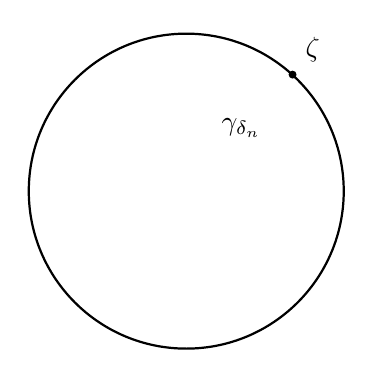
\begin{tikzpicture}[thick]
                \filldraw[black] (1.35,1.48) circle (1pt) node[above right=1pt,fill=white]{$\zeta$};
                \draw (0,0) circle (2cm);
                %\draw [thick,domain=152:303] plot ({1.35 + cos(\x)}, {1.48 + sin(\x)});
                \centerarc[thick](1.35,1.48)(148:307:0.7);
                \node at (0.7,0.8) {$\gamma_{\delta_n}$};
            \end{tikzpicture}
            \label{fig:circle}
        \end{minipage}
        \begin{minipage}[h]{0.5\textwidth}
            \centering
            \begin{tikzpicture}[thick,scale=0.6, use Hobby shortcut,closed=true]
                \filldraw[black] (5.5,6) circle (2pt) node[above = 1pt,fill=white]{$\alpha_n$};
                \filldraw[black] (8,4.5) circle (2pt) node[right = 1pt,fill=white]{$\beta_n$};
                \node[above] at (7.5,5.7) {$\sigma_n$};
                \node[below = 5pt] at (6.5,5.7) {$U_n$};
                \node[below = 5pt] at (6,4.3) {$\varphi(\gamma_{\delta_n})$};
                \draw (1, 0.2) .. (2, 0) .. (3, 1) .. (4, 2.1) .. (5, 2.3) .. (6, 2.4) .. (7, 2.7) .. (7.5, 3) .. (8, 4.5) .. (7, 5.7) .. (5.5, 6) .. (4, 5.7) .. (3, 4.8) .. (2, 4.3) .. (1, 4.2) .. (0.5, 4) .. (0, 2);
                \draw (5.5, 6) .. (5.7, 5.5) .. (5.5, 4) .. (6, 4) .. (7, 3.9) .. (7.5, 4.3).. (8, 4.5);
            \end{tikzpicture}
            \label{fig:jordandomain}
      \end{minipage}
      \caption{Las curvas $\gamma_{\delta_n}$ y $\varphi(\gamma_{\delta_n})$.}
      \label{fig:caratheodory}
    \end{figure}


    Entonces, existe una sucesión $\{ \delta_n\} \downarrow 0$ tal que $L(\delta_n) \to 0$. Cuando $L(\delta_n) < \infty$, la curva $\varphi(\gamma_{\delta_n})$ tiene extremos $\alpha_n, \beta_n \in \xbar{\Omega}$ y ambos puntos deben estar en $\Gamma = \partial \Omega$. De hecho, si $\alpha_n \in \Omega$, entonces algún punto cerca de $\alpha_n$ tiene dos preimágenes distintas en $\disk$ y esto es imposible pues $\varphi$ es inyectiva. Además,
    \begin{equation}\label{res}
        \abs{\alpha_n - \beta_n} \leq L(\delta_n) \to 0.
    \end{equation}

    Sea $\sigma_n$ el subarco cerrado de $\Gamma$ que tiene extremos $\alpha_n$ y $\beta_n$ y con un diámetro menor. Entonces \eqref{res} implica que $\diam(\sigma_n) \to 0$ porque $\Gamma$ es homeomorfa al círculo. Por el teorema de la curva de Jordan, $\sigma_n \cup \varphi(\gamma_{\delta_n})$ divide al plano en dos regiones, y una de ellas, llamémosla $U_n$ es acotada. Entonces $U_n \subset \Omega$ ya que $\complex^* \setminus \xbar{\Omega}$ es conexo por arcos. Como
    \begin{equation}
        \diam(\partial U_n) = \diam(\sigma_n \cup \varphi(\gamma_{\delta_n})) \to 0,
    \end{equation}
    concluimos que
    \begin{equation}
        \label{res2}
        \diam(U_n) \to 0.
    \end{equation}

    Tomamos $D_n = \disk \cup \{ z: \abs{z - \zeta} < \delta_n \}$. Sabemos que para $n$ suficientemente grande, $\varphi(D_n) = U_n$. Si no, por conexión tendríamos que $\varphi(\disk \setminus \xbar{D_n}) = U_n$ y
    \begin{equation*}
        \diam (U_n) \geq \diam (\varphi(B(0, 1/2))) > 0
    \end{equation*}

    que contradice con \eqref{res2}. Entonces $\diam(\varphi(D_n)) \to 0$ y $\bigcap \xbar{\varphi(D_n)}$ es un solo punto pues $\varphi(D_{n+1}) \subset \varphi(D_n)$. Esto significa que $\varphi$ tiene una extensión continua en $\disk \cap \{ \zeta \}$. La extensión a todos estos puntos define una aplicación continua en $\closedisk$. \\

    Denotemos ahora por $\varphi$ a la extensión $\varphi : \closedisk \to \xbar{\Omega}$. Como $\varphi(\disk) = \Omega$, $\varphi$ lleva  $\closedisk$ en $\xbar{\Omega}$. Para probar que $\varphi$ es inyectiva, supongamos que $\varphi(\zeta_1) = \varphi(\zeta_2), \, \zeta_1 \not = \zeta_2$. El argumento utilizado para mostrar que $\alpha_n \in \Gamma$, también prueba que $\varphi (\partial \disk) = \Gamma$, así que podemos suponer que $\zeta_j \in \partial \disk, \, j=1, 2$. La curva de Jordan
    \begin{equation*}
        \{\varphi (r \zeta_1) : 0 \leq r \leq 1\} \cup \{\varphi (r \zeta_2) : 0 \leq r \leq 1\}
    \end{equation*}

    acota al dominio $W \subset \Omega$, luego $\varphi ^{-1} (W)$ es una de las dos componentes de
    \begin{equation*}
        \disk \setminus ( \{ r \zeta_1 : 0 \leq r \leq 1\} \cup \{ r \zeta_2 : 0 \leq r \leq 1\}).
    \end{equation*}

    Pero como $\varphi(\partial \disk) \subset \Gamma$,
    \begin{equation*}
        \varphi(\partial \disk \cap \partial \varphi ^{-1} (W)) \subset \partial W \cap \partial \Omega = \{ \varphi (\zeta_1)\}
    \end{equation*}

    y $\varphi$ es constante en un arco de $\partial \disk$. Se tiene que $\varphi$ es constante, por el principio de reflexión de Schwarz, y esta contradicción prueba que $\varphi(\zeta_1) \not = \varphi(\zeta_2)$. \\
\end{proof}

También podemos utilizar el Teorema de Carathéodory para resolver el problema de Dirichlet como hemos hecho empleando el Teorema de Fatou pero esta vez no necesariamente en el disco unidad. Sea $f$ una aplicación en $\Gamma$ tal que $f \circ \varphi$ es integrable en $\partial \disk$, entonces
\todo[inline]{Revisar}
\begin{equation*}
    u(z) = \dfrac{1}{2 \pi} \int_{- \pi}^{\pi} P_r (\theta - t) f \circ \varphi (e^{it}) dt
\end{equation*}
es armónica en $\Omega$ y por los teoremas \ref{caratheodory} y \ref{fatouaux1},
\begin{equation}
    \label{caratheodoryaux}
    \lim_{z \to \zeta} u(z) = f(\zeta)
\end{equation}
cuando $z \in \Omega$ y la función $f \circ \varphi$ es continua en $\varphi^{-1}(\zeta) \in \partial \disk$. En particular, si $f$ es continua en $\Gamma$, entonces \eqref{caratheodoryaux} se satisface para todo $\zeta \in \Gamma$ y $u(z)$ resuelve el problema de Dirichlet para $f$ en $\Omega$. \\

Al final de la demostración del Teorema \ref{caratheodory} hemos utilizado el resultado que enunciamos a continuación: \\

\begin{theorem}[Principio de Reflexión de Schwarz] Sea $U^+$ un conjunto abierto conexo del semiplano superior y supongamos que la frontera de $U^+$ contiene un intervalo abierto $I \subset \real$. Sea $U^-$ la reflexión de $U^+$ en el eje real, $U^- = \{z: \xbar{z} \in U^+\}$, y  tomemos $U = U^+ \, \cup \, I \, \cup \, U^-$.
    \begin{itemize}
        \item Si $f$ es una función en $U$, holomorfa en $U^+ \, \cup \, U^-$, y continua en $I$, entonces $f$ es holomorfa en $V$.

        \item Si $f$ es una función en $U^+ \, \cup \, I$, holomorfa en $U^+$ y continua en $I$, y toma valores reales en $I$, entonces $f$ tiene una continuación analítica única $F$ en $U$ que verifica
            \begin{equation*}
                F(z) = \xbar{f(\xbar{z})}.
            \end{equation*}

        \item Si $f = u + iv$ es una función holomorfa en $U^+$ y $\lim_{n \to \infty} v(z_n) = 0$ para toda sucesión $\{z_n\}\subset U^+$ que converge a un punto de $I$. Entonces $f$ tiene una continuación analítica única $F$ en $U$ que verifica
            \begin{align*}
                F(z) &= f(z) \text{ si } z\in U^+, & F(\xbar{z}) &= \xbar{F(z)} \text{ si } z\in U.
            \end{align*}
    \end{itemize}
\end{theorem}

El teorema anterior puede aplicarse a situaciones más generales que son isomorfas a la de dicho teorema. \\

\begin{theorem}[Principio de Reflexión de Schwarz] Sea $V$ un conjunto abierto de $\complex$ y supongamos que es la unión disjunta $V = V^+ \, \cup \, \gamma \, \cup \, V^-$, donde $V^+$ y $V^-$ son abiertos de $\complex$ y $\gamma$ es una curva. Suponemos que existe un isomorfismo
    \begin{equation*}
        \psi: U \to V
    \end{equation*}
    tal que
    \begin{align*}
        \psi(U^+) &= V^+, & \psi(I) &= \gamma & \psi(U^-) &= V^-.
    \end{align*}

    La notación $U = U^+ \, \cup \, I \, \cup \, U^-$ es la misma que antes.

    \begin{itemize}
        \item Si $g$ es una función en $V$, holomorfa en $V^+ \, \cup \, V^-$, y continua en $\gamma$, entonces $g$ es holomorfa en $V$.

        \item Si $g$ es una función holomorfa en $V^+$ que se extiende a una función continua en $V^+ \, \cup \, \gamma$, y toma valores reales en $\gamma$, entonces $g$ tiene una continuación analítica en $V$.

        \item Si $g = u + iv$ es una función holomorfa en $V^+$ y $\lim_{n \to \infty} v(z_n) = 0$ para toda sucesión $\{z_n\}\subset V^+$ que converge a un punto de $\gamma$. Entonces $g$ tiene una continuación analítica en $V$.
    \end{itemize}
\end{theorem}


El resultado que presentamos a continuación es un recíproco parcial del teorema de Carathéodory. Muestra que la inyectividad en el borde del dominio se traslada al interior, en condiciones adecuadas. \\

\begin{theorem}
    Sea $\Gamma$ una curva simple, cerrada y suave con interior $\Omega$. Sea $f \in \holomorphic{\Gamma \, \cup \, \Omega}$ una aplicación inyectiva en $\Gamma$. Entonces $f$ es holomorfa e inyectiva en $\Omega$. \\
\end{theorem}

\begin{proof}
    La aplicación $w = f(z)$ lleva $\Gamma$ en un camino simple, cerrado y suave $\Gamma'$. Sea $w_0$ un punto arbitrario que no esté en $\Gamma'$. Entonces, si llamamos $\Gamma_+$ al camino positivamente orientado,
    \begin{equation*}
        n = \dfrac{1}{2 \pi i} \int_{\Gamma_+} \dfrac{f'(z)}{f(z) - w_0} dz =  \dfrac{1}{2 \pi i} \int_{\Gamma'} \dfrac{dw}{w - w_0}.
    \end{equation*}

    Ahora la última integral es cero si $w_0$ está fuera de $\Gamma'$ y es $\pm 1$ si $w_0$ está dentro de $\Gamma'$. Sin embargo, $n$ no puede ser negativo pues la primera integral nos da el número de ceros de $f(z) - w_0$ dentro de $\Gamma$. Entonces, $n=1$ si $w_0$ está dentro de $\Gamma'$. \\

    Esto prueba que $f(z) = w_0$ tiene una sola solución si $w_0$ está dentro de $\Gamma'$, que $f(z)$ es holomorfa e inyectiva en $\Omega$ y lleva $\Omega$ en $\Omega'$ (el interior de $\Gamma'$) y que la dirección positiva de $\Gamma'$ se corresponde con la dirección positiva de $\Gamma$.
\end{proof}

